\subsubsection{Board Representation}

Since the computer cannot work with a physical chess board and pieces, these must be converted into a form in which the board, pieces, and position can be interpreted by the computer and later used for the input layer of the neural network. The most common form of representation is the data structures bitboards. A bitboard is implemented as an $8 \times 8$ array, which is the size of a chessboard. Each array element corresponds to a square on the board. A bitboard is created for each type of piece (pawn, knight, bishop, rook, queen and king) of a given color (black and white). This gives a total number of 12 bitboards. Finally, the squares on which the figures are placed must be marked on the respective boards. This can be done in binary, where 0 means the square is empty and 1 means the square is not empty.

\begin{figure}[h]
\centering
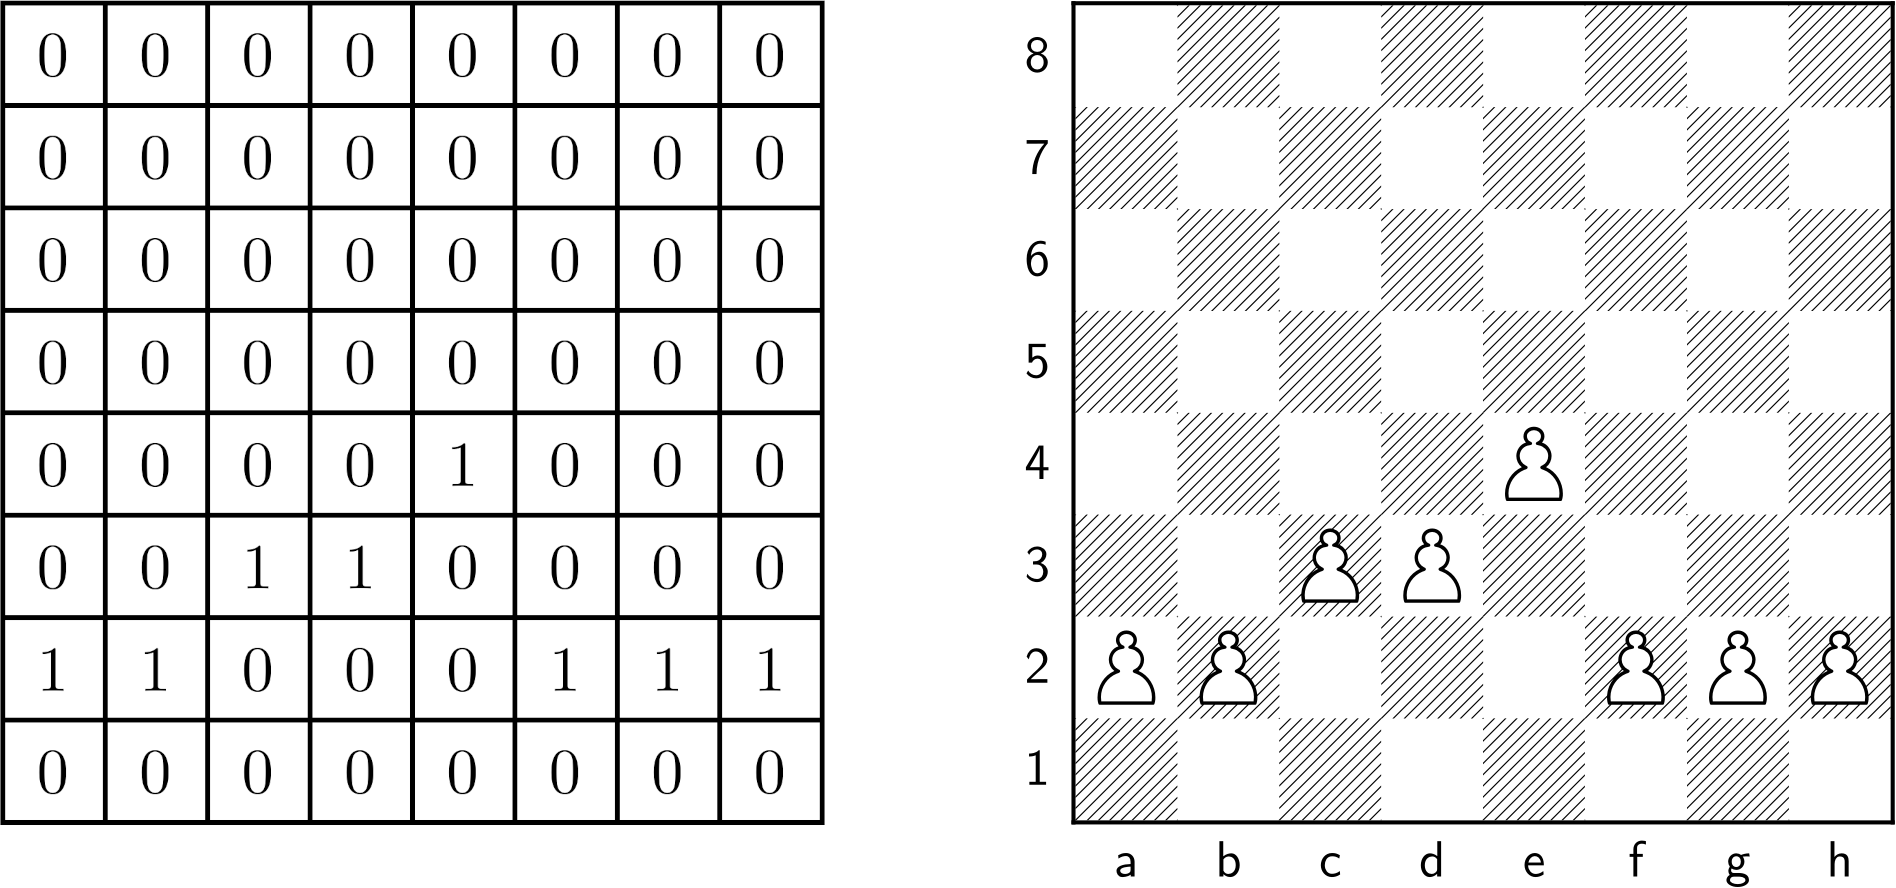
\includegraphics[scale=0.13]{graphics/bitboard/bitboard_and_chessboard.png}
\caption{Representation of bitboard with white pawns (left) and the corresponding chessboard (right)}
\end{figure}

Through the usage of the logical operations, such as AND, OR, NOT the moves can be calculated. An advantage of the logical operations is, that be done quite fast by the processor. Furthermore, with x64 processors the position can be stored in one piece in the memory, as a bit string, since this is exactly 64 bits long due to the number of squares. Another advantage is that due to its simple representation, it can be used as input for the input layer in the neural network without the need to convert it into an understandable format.